\section{Introduction}
\label{sec-introduction}

% introduce LPL asynchronous duty cycle media access
As already we are aware, smartphones have become a necessity in our lives, as we are checking our mobile phones constantly throughout the day. As a result, some concerns of privacy have arisen about nearby parties peeking at our screen, or ‘shoulder surfing’. Although great effort has been put forward to mitigate this threat, from physical privacy films to alternative password entry interfaces \cite{wiedenbeck2006design} \cite{papadopoulos2017illusionpin} and input methods \cite{kumar2007reducing}, these methods often require additional cost and/or effort \cite{Chun2019Keep} and are not widely implemented yet on the privacy critical stages (e.g. password entry) of most everyday apps.

On the other hand, many works in this area are built on a threat model of an attacker observing with his/hers naked eye, as they assume that the attacker is not malicious and merely take several peeks out of curiosity. Although studies have shown that a great portion of these attacks are casual and opportunistic without technical equipment\cite{eiband2017understanding}, however, a mere stranger can hardly do any harm reading a fragment of your correspondence or acquiring your password without knowing your account(which, in critical apps like Alipay, seldom appears on screen in common usage). It is the rare but malicious attacker, with certain familiarity and knowledge of the victim, that can do the most harm. The attacker can even be our closest friends or family members, as there are various cases in China where a child obtains Alipay password of their parents, and, unaware that electronic payments consists of 'real' money, ends up spending them lavishly in their games. What's more, specially made equipment are not a necessity for these attacks to happen. If we only equip the observer with a smartphone, he/she can not only acquire sensitive information from long distances, reducing suspicion, but also record the information for propagating, dealing greater damage to the victim. For example, in a Senate hearing, the Justice Secretary of Philippines, Vitaliano Aguirre II, suffered a leakage of his text messages, as someone had taken a snapshot of his smartphone \cite{Polotiko2017leakage}. Moreover, smartphones have seen great improvement these years. Equipped with multiple cameras, the newest generation of smartphones can perform 100x zooming compared to the standard 5x of single camera phones. Improvements in memory hardware also allows burst mode at tremendous frame rates and even high-speed photography, recording videos with thousands of frames per second, and more images means more information. By capturing multiple images of the victim's phone, and processing them with multi-frame super resolution (SR) methods, the attacker can gain vital data from even further away. In this present era where the leakage of a password can cost thousands, and the disclosure of correspondence of public figures can cause huge sensations in media and great damage to the victim, we believe that it's imminent to recall attention on this privacy threat and propose a new standard of screen protection based on modern circumstances.
 
While exploring this privacy threat, we need to implement a multi-frame SR algorithm on a smartphone in order to monitor the target phone in real time. However, we discovered that there is no published SR algorithm suitable for this scenario. Apparently, the blurriness of the images calls for deep-learning based methods, however most of these methods function on a handful of clearer images(scenary, scanned images, etc.) \cite{nasrollahi2020deep} \cite{lyn2020image}, but we have to merge the information from large quantities of extremely blurred photos, as smartphones can capture 100 snapshots in a few seconds in burst mode, and these photos are taken from extreme distances(to test the theorectical limits of the privacy threat). The different nature between videos and multiple snapshots also rules out the video super resolution methods. The algorithms cannot be adapted to function on larger numbers of input images, because 1) either increased input leads to increases in model complexity, making it unsuitable for mobile deployment, or 2) they lack emphesis on the process of horizontal comparison, relying heavily on the information extracted from each single image, and thus merges the information inefficiency and show unsatisfactory performance. 

To explore this privacy threat and to fill the gap in deep-learning based multi-frame super resolution, we designed an end-to-end CNN-based architecture for shoulder surfing and similar multi-frame SR applications with massive input and blurry images. To utilize the large amount of data with low computational complexity, we designed a unique merging layer and placed it between convolutional layers in the SR pipeline. The input images are processed independently and the information extracted are then merged together, serving as a reference for the following convolutions. With the network as core, We then implemented a holistic system for shoulder surfing on a smartphone, which captures multiple images in burst mode, process them with our neural network to generate a high-res image, and repeating this process for constant monitoring. As the information of interest is mostly in the form of text (e.g. passwords or e-mails), our network is trained and evaluated on the task of reconstructing text, specifically, Chinese characters, English letters, and numbers, but we believe that this network architecture can function in all scenarios. Our system can also be used as a preprocessor for text-recognition applications when multiple images are available, such as real-time translation apps on a smartphone or text-recognition on self-driving cars.

\subsection{Difficulties}
There are several difficulties unique to this SR application. The most prominent one is the blurriness, as our photos are taken at extreme range, taken secretly and hurriedly without much room for focusing, while straining the magnification of the smartphone lenses. Unlike most SR applications and datasets working with ‘normally’ captured photos, the images we face exhibit lower concentrations of information and more artifacts, and needs more ‘reconstruction’ than ‘interpolation’.

Another difficulty unique to our task is the subject—mainly, Chinese characters. Composed of multiple strokes, these characters are distributed discretely in image space, not known to other entities, e.g. faces and natural objects. In some cases, messing up a stroke will not impact its readability, and in other cases shortening or lengthening a stroke even slightly will lead to a different character, leading to misunderstandings. And unlike most SR applications working on similarity (between their output and the ‘ground truth’), our goal is readability, and the network architecture and training process must be engineered accordingly.
 
\begin{figure}
	\centering
	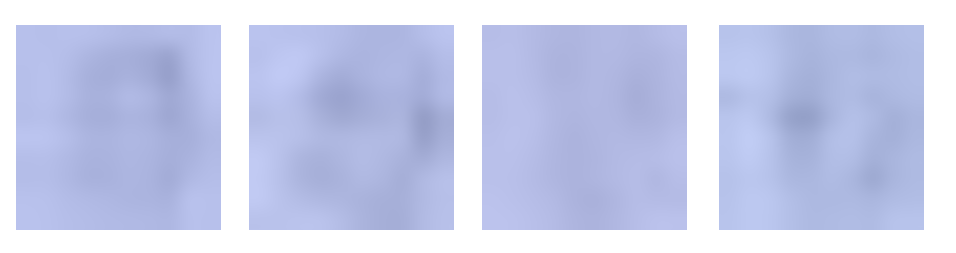
\includegraphics[width=0.48\textwidth]{pic/zeros}
    \caption{ Fig 1. 4 photos of number ‘0’ on a screen at a distance of 1.5m, taken in quick succession from a still smartphone camera. Note how they exhibit different blurriness and display no consistency between neighboring frames.}
	\label{fig-zeros}
\end{figure}


\subsection{Network Architecture} 
 As mentioned above, reconstructing images with high degrees of blurriness requires a unique approach. Most works on multi-frame SR function on video clips \cite{lucas2019generative} or multiple snapshots \cite{wronski2019handheld}, however, our application is subtly different from the two. Our dilemma is as follows: on one hand, each one of the photos we are to process is blurred with a randomly different PSF kernel, which, because of the extreme blurriness, cannot be approximated as a constant, isotropic gaussian kernel, and thus lacking consistency between neighboring frames, meaning that they cannot be processed as a video clip(see Figure~\ref{fig-zeros} ); on the other hand, because of the low concentration of information, the blurred photos are similar to pieces of a jigsaw puzzle, each containing only fractions of information, and the only chance of recovering the ground truth is by comparing each photo against others. If processed by common procedures enhancing the resolution of a series of snapshots—processing each one separately and merging them afterwards, few useful information can be extracted from each one of the images, and merging them will not produce satisfactory results.

Considering the unique challenges of our application, we believe that if these images are processed iteratively, alternating between the following two processes, our network will be able to solve this ‘jigsaw puzzle’:

\begin{enumerate}
  \item Every single image of the input collection will be processed solely (by several layers of CNN), with access of the output of step (2) of the last iteration;
  \item The processed results will be merged (with weighted averaging methods) and distributed to each photo for the next iteration.
\end{enumerate}

This architecture is beneficial to our task. On one hand, the deep learning part is assigned to each single image, reducing computational complexity and parameter growth, while receiving a global view of all the images, renewed at each layer, thanks to the merging process; on the other hand, information can be shared horizontally with weighted averaging methods, meaning no consideration of sequential order and no reliance of consistency between neighboring frames. Thus, this architecture solves the dilemma mentioned above, and proves perfectly functional in our application.

The details of our architecture will be discussed in section 4.

This paper makes the following contributions:

\begin{itemize}
  \item	We propose SRPeek, a multi-frame SR neural network architecture aiming at reconstructing extremely blurred and defocused images. This model is not only functional in our scenario, as a shoulder-surfing threat model, but also can be used in text-recognition applications prior to recognition algorithms to increase accuracy.
  \item	We design a threat model of shoulder-surfing, with the attacker armed with multi-frame SR algorithms and taking multiple photos (in burst mode) of the victim’s screen with a smartphone camera. To the best of our knowledge, we are the first to consider the presence of smartphone cameras and SR algorithms in shouler surfing senarios.
  \item	We demonstrate the effect of this shoulder-surfing attack and prove that it poses a threat to screen privacy.
\end{itemize}

% describe the organization of the paper
The rest of the paper is organized as follows. Section 2 describes the threat model of our  carefully studies the performance of state-of-the-art concurrent flooding. The detailed design of COFlood protocol is shown in Section~\ref{sec-design}. We show the implementation details and evaluation results in Section~\ref{sec-implementation-and-evaluation}. The related work is introduced in Section~\ref{sec-related-work}. Finally, we conclude our work in Section~\ref{sec-conclusion}.
